\chapter{Tree Edit Distance}
In this chapter we will discuss the so called \textit{tree edit distance}. This chapter is based on Demaine et al.'s paper about an optimal decomposition algorithm []. 

\section{Introduction} 
\begin{defin} \label{def:ted}
Let $T_1=(V_1,E_1)$ and $T_2=(V_2,E_2)$ be two rooted ordered labelled trees together with a set of labels $\Sigma$. Furthermore let the costs for the basic edit operations relabelling, inserting and deleting be fixed. \\
Let $o^*:= (o^*_1,...,o^*_n)$ be a finite sequence of edit operations that fulfills the following:
\begin{align*}
o^*(T_1) &= o^*_n(...(o^*_1(T_1)) = T_2 \\
c(o^*) = \sideset{}{}\sum_{i=1}^n c(o^*_i) &= \sideset{}{}\min_{\substack{o\text{ sequence of}\\ \text{edit operations}}} \{c(o)\,|\,o(T_1)=T_2\}
\end{align*}
Then the \textit{tree edit distance} $\delta(T_1,T_2)$ is defined as:
$$\delta(T_1,T_2) := c(o^*).$$
\end{defin}
\begin{defin}
Let $T_1=(V_1,E_1)$ and $T_2=(V_2,E_2)$ be two rooted ordered labelled forests and the rest as in the definition~\ref{def:ted}. Then we can extend the definition of the tree edit distance $\delta(T_1,T_2)$ trivially. 
\end{defin}

The origin of finding the tree edit distance is an intuitive way of comparing two trees. Given two labelled ordered trees $T_1$ and $T_2$. What is the cheapest sequence of edit operations that transforms $T_1$ into $T_2$? Take a look at the trees $T_1$ and $T_2$ in~\ref{fig:TEE} and the sequence of operations that performs the transformation from $T_1$ to $T_2$. If we assume, for example, that every operation costs the same then the sequence shown in the figure would be an optimal one.
\begin{figure}[!h]
    \centering
    \begin{subfigure}[b]{\textwidth}
		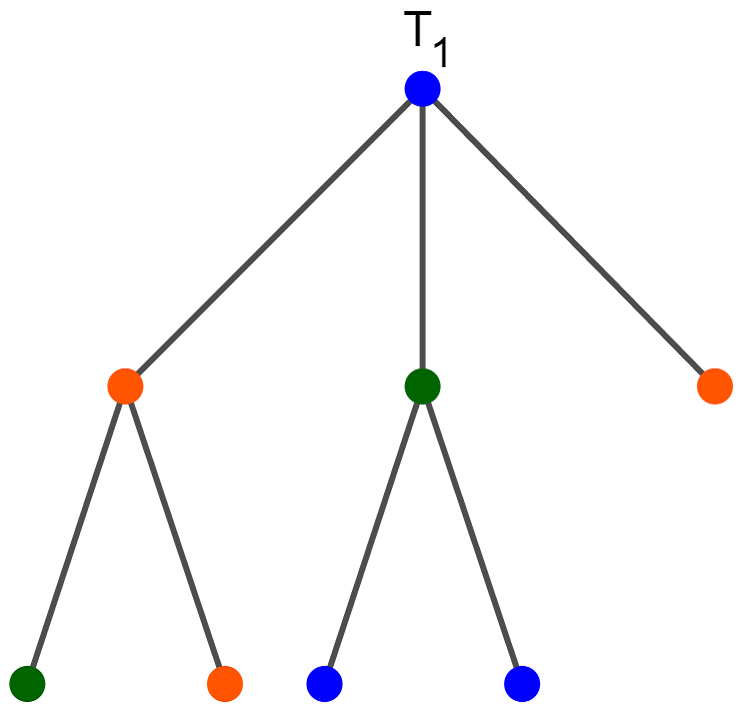
\includegraphics[width=0.39\textwidth]{figures/TreeEditExample_1.jpg}
		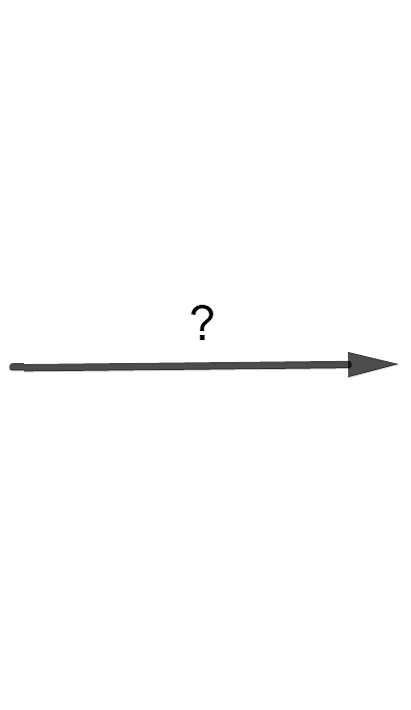
\includegraphics[width=0.2\textwidth]{figures/TreeEditExample_1,5.jpg}
		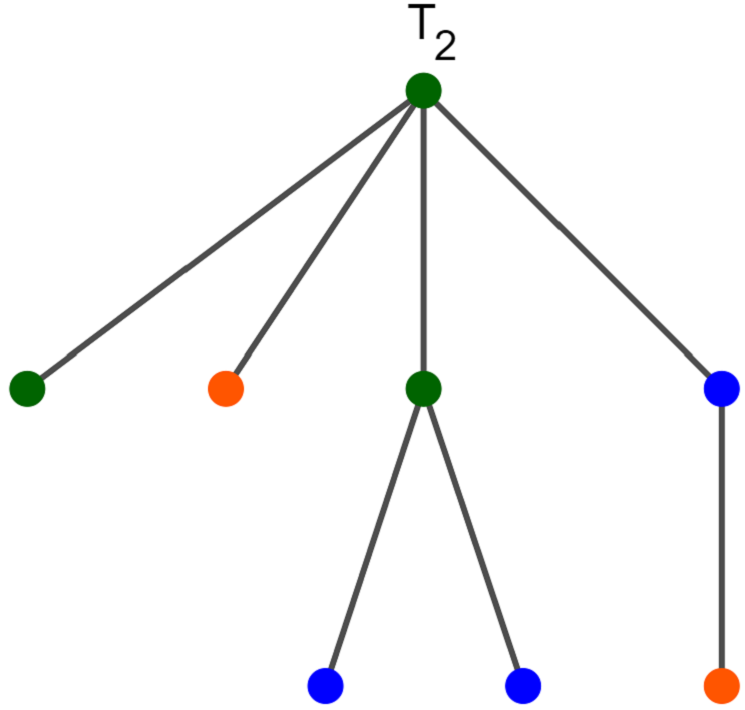
\includegraphics[width=0.39\textwidth]{figures/TreeEditExample_2.jpg}
		\caption{Consider these two trees $T_1$ and $T_2$. Finding the cheapest way of transforming $T_1$ into $T_2$ can be really hard. Underneath we see one sequence of editing operations that could be the cheapest one.}
	\end{subfigure}
    \begin{subfigure}[b]{\textwidth}
		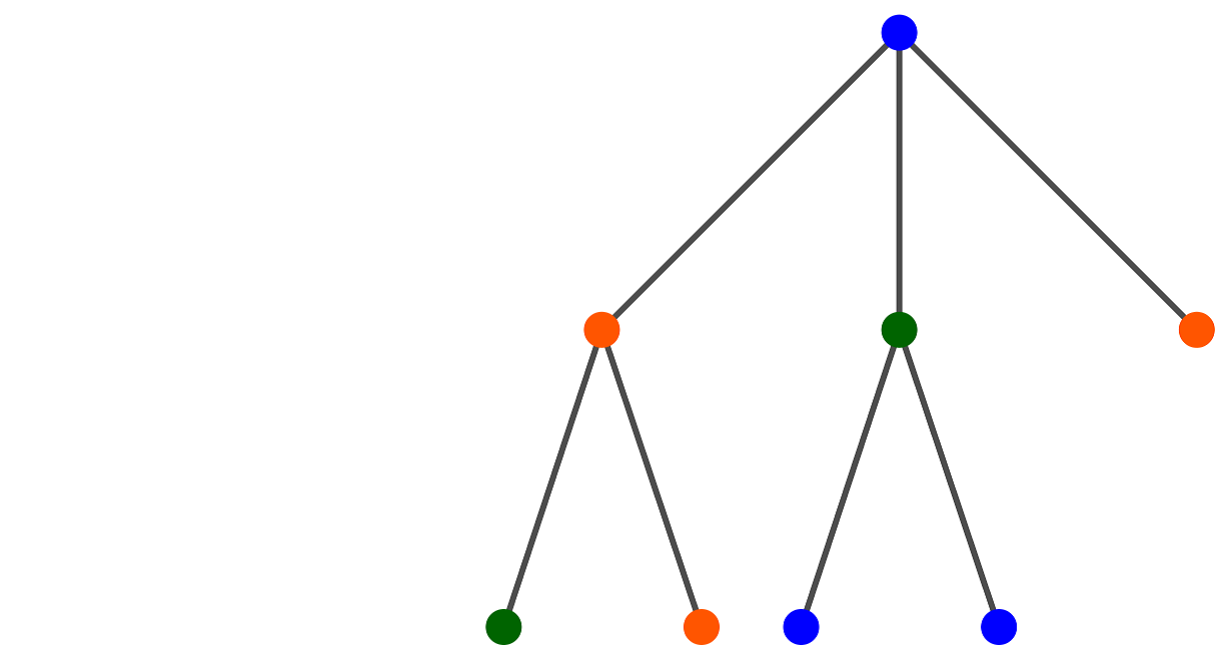
\includegraphics[width=0.45\textwidth]{figures/TreeEditExample_3.jpg}
		\quad
		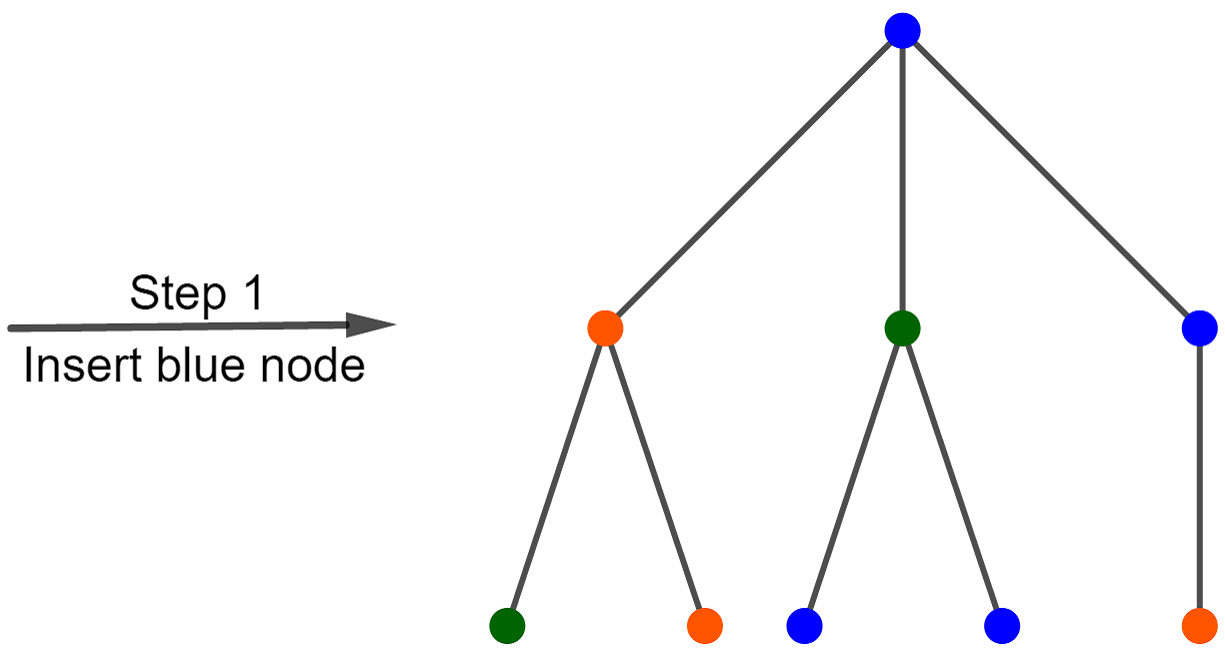
\includegraphics[width=0.45\textwidth]{figures/TreeEditExample_4.jpg}
		\\ %comment
		\\
		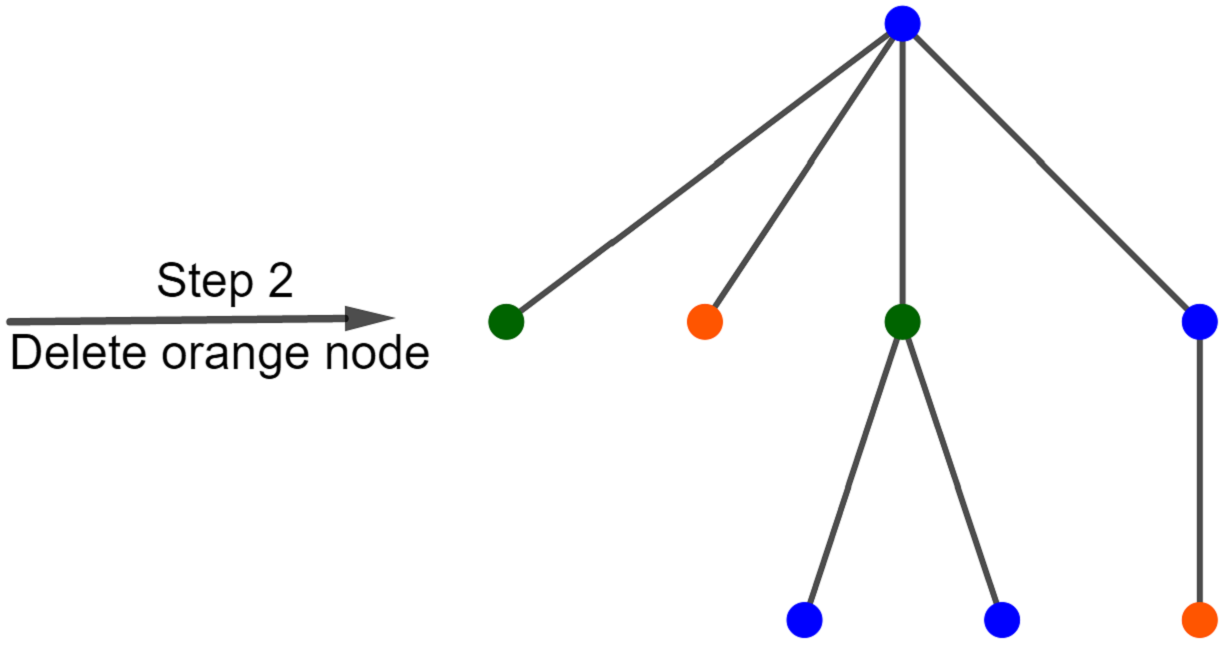
\includegraphics[width=0.45\textwidth]{figures/TreeEditExample_5.jpg}
		\quad
		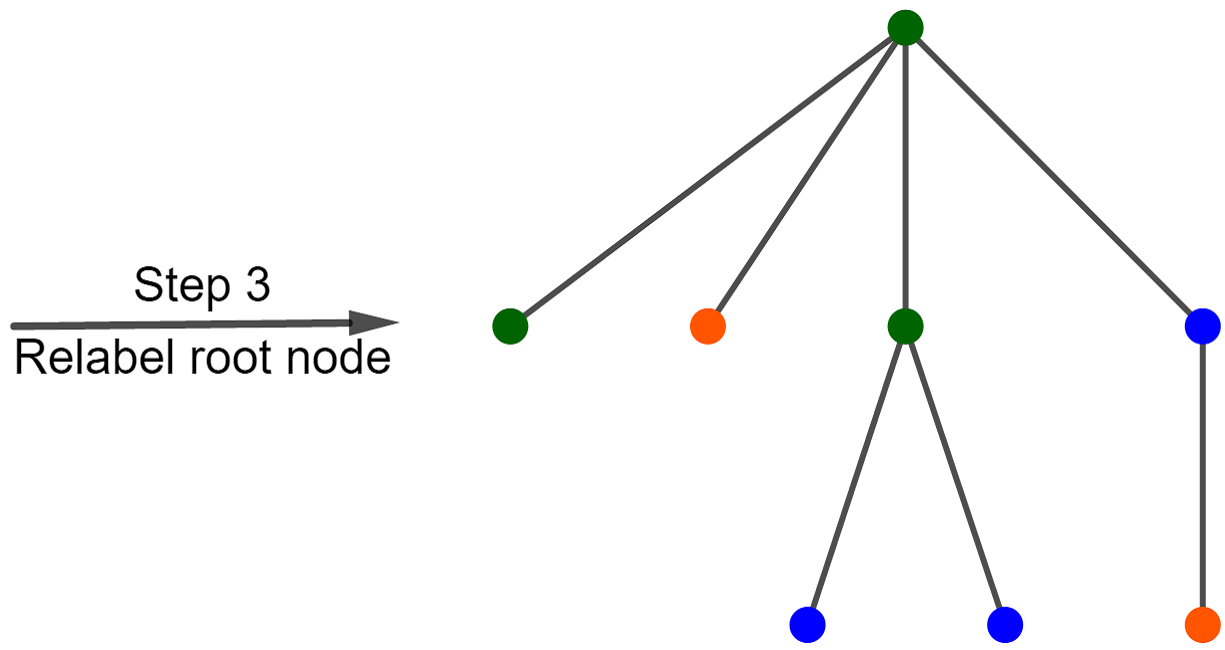
\includegraphics[width=0.45\textwidth]{figures/TreeEditExample_6.jpg}
		\caption{Step 1: Insert a node right above the rightmost child of the root. Step 2: Delete the leftmost child of the root. Step 3: Relabel the root node.}
	\end{subfigure}
	\label{fig:TEE}
\end{figure}
The tree edit distance is used in the fields of structured text databases, computer vision and in bioinformatics. In the last field one needs to compare the secondary structure of RNA-molecules without the disadvantages of other approaches. For a more detailed description about this topic please take a look at [].

\section{Short History of the Tree Edit Distance}
The tree edit distance was introduced by Tai in the year 1979~\cite{Tai}. In addition to the definition he also provided an algorithm to compute the tree edit distance. The running time and space complexity amounts to $O(t_{l,1}^2 t_{l,2}^2 t_1 t_2)$ which implies a worst-case running time of $O(t_1^6)$. \\
It took about a century until Shasha and Zhang~\cite{SasAndZha} came up with a dynamic programming approach that improved the running time to $O(t_1^2 t_2^2)$. Later on Klein~\cite{Kle} started with his algorithm, changed the way to of branching and was able to further improve the running time to $O(t_1 t_2^2 \log t_1)$ time. Dulucq and Touzet~\cite{DulAndTou} proved a lower bound of $\Omega(t_1 t_2 \log t_1 \log t_2)$ on the running time for all algorithms for the tree edit distance which are based on dynamic programming in 2003. Finally, in 2007 Demaine et al.~\cite{Dem} provided an algorithm that satisfies the lower bound on dynamic programming approaches.\\
Chen~\cite{Che} presented a different approach relying on fast matrix multiplication solving the tree edit distance problem in $O(t_1 t_2 + t_1 t_{2,l}^2 + t_{1,l}t_{2,l}^{2.5})$ time and $O(t_1 + (t_2 + t_{2,l}^2)\min \{t_{1,l},t_{2,l}\})$ space. You can also take a look at other algorithms, see~\cite{Apo, Bil, Val}

In this thesis we will concentrate on the dynamic programming approaches of Shasha and Zhang, Klein and last but not least Demaine et al. But since this thesis tries to show different comparing mechanisms we will keep it rather short. If you want to have a more detailed description about something, please take a look into the original papers.

\section{Dynamic Programming Approach}
The key for any dynamic programming approach is to find a suitable way for branching a hard problem into smaller and therefore easier subproblems. 
\begin{defin}
Let $T_1,T_2$ be two rooted labelled ordered forests and let the cost functions be defined as stated in the definition.
Consider the problem of computing $\delta(T_1,T_2)$ with a fixed dynamic programming approach $A$. A \textit{relevant subproblem} of $(T_1,T_2)$ is any pair of rooted labelled forests $(T_1',T_2')$ such that the following holds:\\
During the computation of $\delta(T_1,T_2)$ we encounter the problem of solving $\delta(T_1',T_2')$. We define $\mathcal{R}_A$ to be the set of all relevant subproblems\\
We call $(T_1',T_2')$ to be a trivial subproblem if and only if $(T_1',T_2')$ is a relevant subproblem and $\exists i \in \{1,2\}$ s.t. $T_i' = (\emptyset,\emptyset)$. We defnine $\mathcal{T}_A \subset \mathcal{R}_A$ to be set of all trivial subproblems.
\end{defin}
\begin{rem}
Since a relevant subproblem $(T_1',T_2')$ occurs in the computation of $\delta(T_1,T_2)$, there has to exist a sequence of basic editing operations $o$ only consisting of relabelling and deleting operations s.t. $o(T_1)=T_i' \, \forall i \in \{1,2\}$.
\end{rem}
\begin{rem}
We only consider deleting and relabelling operations because of the symmetry between deleting a node in $T_1$ and inserting a proper node in $T_2$ vice versa.
\end{rem}
\begin{rem}
A trivial dynamic programming approach would lead to $\Omega(2^{t_1+t_2})$ subproblems. Therefore it is necessary to branch in a smart way to get a polynomial number of relevant subproblems.
\end{rem}
The idea of branching is to consider the two rightmost or leftmost roots of $T_1$ and $T_2$. Either one of those two gets deleted or the two roots are matched. In the first case you result in a new smaller relevant subproblem, in the latter you even end up with two separated relevant subproblems:\\
Suppose you match $r_{T_1}$ with  $r_{T_2}$. Then any node from $R_{T_1}$ that gets matched with a node in $T_2$ has to be matched with a node in $R_{T_2}$ because of the strict ancestry relation. So matching those two roots splits the problem of computing $\delta(T_1,T_2)$ into the two subproblems of computing $\delta(R_{T_1}^{\circ},R_{T_2}^{\circ})$ and $\delta(T_1-R_{T_1},T_2-R_{T_2})$.
\begin{defin}
Consider the problem of computing the tree edit distance $\delta(T_1,T_2)$ with a dynamic programming approach $A$.\\
We call $S_A : \mathcal{R}_A \mapsto \{\text{left,right}\}$ the \textit{decomposition strategy} of the dynamic programming approach $A$ if for any relevant subproblem  $(T_1',T_2') \in \mathcal{R}_A$ the following holds: \\
The direction $S_A((T_1',T_2'))$ coincides with the direction of branching according to the dynamic programming approach $A$.
\end{defin}


\subsection{Shasha and Zhang's algorithm}\label{sec:saz}
Shasha and Zhangs algorithm is the most basic dynamic programming approach. They restrict themselves to the decomposition strategy that always chooses the right direction. 
\begin{lem}\label{lem:sets}
Let $T_1,T_2$ be two rooted labelled forests and assume these forests are ordered according to the post order indexing. Consider the problem of computing  $\delta(T_1,T_2)$ with a dynamic programming approach $A$ that has a decomposition strategy $S_A(T_1',T_2') = \text{right} \, \forall (T_1',T_2') \in \mathcal{R}_A \setminus \mathcal{T}_A$. Then:\\
$\forall (T_1',T_2') \in \mathcal{R}_A \setminus \mathcal{T}_A : \exists \, i_1 \leq j_1,\, i_2 \leq j_2 \in \mathcal{N}$ s.t.:\\
 \begin{align*}
 V(T_1') &= \{i_1,i_1+1,...,j_2\} \\
 V(T_2') &= \{i_2,i_2+1,...,j_2\}.
 \end{align*}
\end{lem}
\begin{rem}[Remark 1]
Because of the post order indexing, the rightmost root $r_T$ has the highest overall index.
\end{rem}
\begin{rem}[Remark 2] 
For two induced subtrees $T_{v'}$ and $T_{v''}$ of $T$ s.t. $V(T') \cup V(T'') = \emptyset$ assume that $v'$ lies on the left of $v''$. Then the index of every node in $T_{v'}$ is strictly smaller than the index of all nodes in $T_{v''}$.
\end{rem}
\begin{proof}
We make an inductive argument. We start with our base: For $T_1$ and $T_2$ the claim is trivially true. So let's consider an induction step and assume that the claim holds for a relevant subproblem $(T_1',T_2')$. Therefore there exists the indexes $i_1,j_1,i_2,j_2$ as in the lemma. We have three possible induction steps:
\begin{enumerate}
\item \textit{Delete $r_{T_1'}$:} If $i_1 \leq j_1-1$ the new indexes will be $i_1,j_1-1,i_2,j_2$ because of Remark 1. Otherwise we just deleted the only node left in $T_1' \Rightarrow $ the new relevant subproblem $(T_1'',T_2'') \in \mathcal{T}_A$
\item \textit{Delete $r_{T_2'}$:} Equivalent to the previous case.
\item \textit{Match $r_{T_1'}$ and $r_{T_2'}$:} As written previously we split the problem $(T_1',T_2')$ into two subproblems $\delta(R_{T_1}^{\circ},R_{T_2}^{\circ})$ and $\delta(T_1-R_{T_1},T_2-R_{T_2})$. Assume both subproblems are not trivial. Using Remark 2 we see that all nodes in $R_{T_1}$ have a higher index than all the nodes in $T_1-R_{T_1}$.\\
$ \Rightarrow \exists k_1$ s.t. $i_1 < k_1 < j_1$ with $V(T_1-R_{T_1})=\{i_1,...k_1-1\}$ and $V(R_{T_1}) = \{k_1,...,j_1\}$ and $k_2$ equivalently,  closing our induction step argument.
\end{enumerate}
\end{proof}
Lemma~\ref{lem:sets} provides us with a trivial upper bound of relevant subproblems of $O(t_1^2t_2^2)$ since there are only $\binom{t_1}{2} = O(t_1^2)$ such sets for $T_1$ and $\binom{t_2}{2} = O(t_2^2)$ such sets for $T_2$ respectively.
\begin{lem}\label{lem:saz}
Let $T_1$, $T_2$ be two rooted ordered labelled forests with the set of labels $\Sigma$. Assume that the cost functions for the basic tree edit operations are fixed. Then one can compute $\delta(T_1,T_2)$ considering $O(\min \{t_{1,l},t_{1,h}\} \min \{t_{2,l}, t_{2,h}\}t_1t_2)$ subproblems with the following recursion steps:
\begin{enumerate}
\item $\delta(\emptyset,\emptyset) = 0$;
\item $\delta(T_1,\emptyset) = \delta(T_1 - r_{T_1},\emptyset)+c_{del}(r_{T_1})$;
\item $\delta(\emptyset,T_2) = \delta(\emptyset, T_2 - r_{T_2})+c_{del}(r_{T_2})$;
\item \[ \delta(T_1,T_2) = \min
	\begin{cases}
	\delta(T_1 - r_{T_1},T_2)+c_{del}(r_{T_1})\\
	\delta(T_1,T_2 - r_{T_2})+c_{del}(r_{T_2})\\
	\delta(R_{T_1}^{\circ},R_{T_2}^{\circ}) + \delta(T_1 - R_{T_1},T_2 - R_{T_2} + c_{rel}(r_{T_1},r_{T_2})
	\end{cases} \]
\end{enumerate}
\end{lem}
\begin{proof}
\textit{Correctness: } Constraint 1 is trivial. Constraints 2 and 3 handle the case of trivial subproblems: We just delete all nodes and add the costs for doing so. For a non-trivial relevant subproblem we have to find the cheapest way of procedure: Either delete a rightmost root or match them. The equations are trivial. 

\textit{Running time: }We calculate an upper bound on the number of different subforests of $T_1$ and $T_2$ that appear in any relevant subproblem independently and multiply those bounds together. Thus we get an overall upper bound on the number of relevant subproblems.\\
For that we have to take a closer look at the role of keyroots and prefixes as defined in the first chapter: Suppose $T_1'$ is a subforest of $T_1$ that appears in some subproblem $\Rightarrow \exists i_{T_1'}, j_{T_1'}$ s.t. $V(T_1')=\{i_{T_1'},...,j_{T_1'}\}$. \\
If $i_{T_1'} = 1$ then, under the assumption that $j_{T_1'} < t_1$, $T_1'$ is a prefix of $T_1^{\circ} = (T_1)_{r_1}^{\circ}$ where $r_1$ is the root of $T_1$.\\
If $i_{T_1'} > 1$ then there has to exist an induced subtree that lies completely on the left of $T_1'$, even if it is only the leftmost leaf. Therefore there exists a biggest subtree that lies completely on the left of $T_1'$. This subtree will be of the form $(T_1)_v$ for some $v \in V(T_1)$. Thus $T_1'$ has to be a prefix of the right sibling $w$ of $v$.\\
In both cases we end up with the statement, that any subforest of $T_1$, appearing in a relevant subproblem, is a prefix of an induced subtree $(T_1)_v$ for some $v \in \text{keyroots}(T_1)$. This implies summing up all such prefixes will be an upper bound on the number of relevant subproblems:
$$\sideset{}{}\sum_{v \in \text{keyroots}(T_1)} |(T_1)_v^{\circ}| = \sideset{}{}\sum_{v \in T_1} \text{cdepth}(v) \leq \sideset{}{}\sum_{v \in T_1}\text{cdepth}(T_1)= |T_1|\text{cdepth}(T_1)$$
Shasha and Zhang went on to prove the missing inequality:
$$\text{cdepth}(T_1) \leq \min \{t_{1,l}, t_{1,h}\}$$
Combining all the parts together we reach target running time of $O(\min \{t_{1,l},t_{1,h}\} \min \{t_{2,l}, t_{2,h}\}t_1t_2)$.
\end{proof}

\subsection{Klein's algorithm}
Klein~\cite{Kle} improved the algorithm of Shasha and Zhang by using a more advanced decomposition strategy. The idea is to compare the sizes of the two outermost trees of $T_1$:
\begin{defin}
Let $(T_1',T_2')$ be any relevant subproblem for computing $\delta(T_1,T_2)$. Klein's decomposition strategy $S_K$ is defined as follows:\\
$$ S_K(T_1',T_2') = 
\begin{cases}
\text{left} & |V(L_{T_1'})| \leq |V(R_{T_1'})| \\
\text{right} & \text{otherwise} 
\end{cases}$$
\end{defin}
Klein's algorithm improved the running time of decomposition algorithms to $O(n^3\log n)$. The proof of this running time makes use of the heavy path decomposition and an upper bound of $\log(T) + O(1)$ on the ldepth$(v)$. The key idea is that every relevant subproblem can be obtained by some $i<|T_v|$ consecutive deletions from $T_v$ for some light node $v \in V(T)$.

\subsection{Demaine et al.'s optimal Algorithm}
Demaine et al. presented a new algorithm based on the dynamic programming approach. They proved a running time of $O(t_2^2t_1(1+\log \frac{t_1}{t_2}))$ and lastly showed that this satisfies a lower bound on the running time of dynamic programming approaches for the tree edit distance.\\
This subsection contains statements without proofs for the sake of this thesis length. If you are interested in them, we would like to refer to the original paper of Demaine et al.~\cite{Dem}
\begin{defin}
Let $(T_1',T_2')$ be any relevant subproblem for computing $\delta(T_1,T_2)$. Demaine et al.'s decomposition strategy $S_D$ is defined as follows:\\
$$ S_D(T_1',T_2') = 
\begin{cases}
\text{left} & \text{if }T_1' \text{ is a tree or if }l_{T_1'} \text{ is not the heavy child of its parent} \\
\text{right} & \text{otherwise} 
\end{cases}$$
\end{defin}
\begin{figure}\label{fig:S_D}
	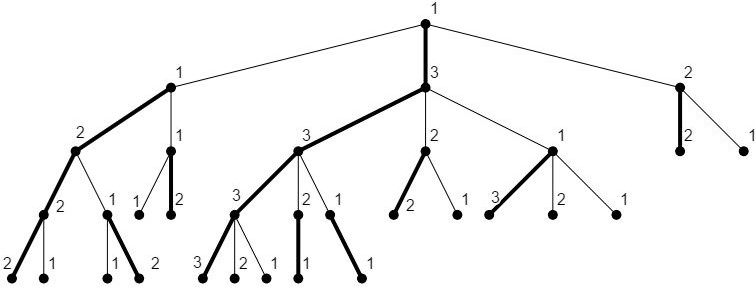
\includegraphics[height=5cm]{figures/optimal_algorithm.jpg}
	\caption{The number at each node indicates the order among siblings in which they are considered according to $S_D$.}
\end{figure}
\begin{rem}
Take a look at Figure~\ref{fig:S_D}. As the caption explains the number at each node shall demonstrate the order among children. If you take a look at the children of the root, for example, the first direction according to $S_D$ would be left, the second one would be right and last but not least the heavy child of the root would be considered.\\
It is trivial, that according to $S_D$ the heavy child of a node will always be considered at last.
\end{rem}
\begin{lem}
Let $T_1,T_2$ rooted ordered labelled trees be given. Suppose we want to compute $\delta((T_1)_v,T_2)$ with $v \in$ TopLight$(T_1)$. Then we encounter all pairs $((T_1)_u^{\circ}, (T_2)_w^{\circ})$ where $u \in T_1, w \in T_2$ and both not on the main heavy paths of $T_1, T_2$ respectively as relevant suproblems and therefore compute $\delta((T_1)_u^{\circ}, (T_2)_w^{\circ}).$ 
\end{lem}

Combining this lemma and the decomposition strategy $S_D$ leads to the following algorithm:
\begin{thm}
We compute $\delta(T_1, T_2)$ recursively as follows:
\begin{enumerate}
\item If $|V(T_1)| < |T_2|$ compute $\delta(T_2, T_1)$ instead.
\item Recursively compute $\delta((T_1)_v,T_2) \, \forall v \in$ TopLight$(T_1)$ using these recursive steps.
\item Compute $\delta(T_1, T_2)$ using the decomposition strategy $S_D$. However do not recurse into subproblems that have previously been computed in step $2$.
\end{enumerate}
Using these steps, we can compute $\delta(T_1,T_2)$ in $O(t_2^2t_1(1+\log \frac{t_1}{t_2}))$ time.
\end{thm}

\subsection{Lower bound on Decomposition Algorithms}
The potential of decomposition algorithms has a bound that has already been achieved by the previous algorithm of Demaine et al. To finish this chapter on the tree edit distance we will present a proof of a lower bound of $\Omega(t_2^2t_1)$ and illustrate the structure of trees which are used to show the actual lower bound of $\Omega(t_2^2t_1(1+\log \frac{t_1}{t_2}))$.
\begin{lem}
For any decomposition algorithm solving the tree edit distance problem,
there exists a pair of trees $(T_1,T_2)$ with sizes $t_1, t_2$ resprectively, such that the number of relevant subproblems is $\Omega(t_2^2t_1)$
\end{lem}
\begin{figure}[!ht]
	\centering
	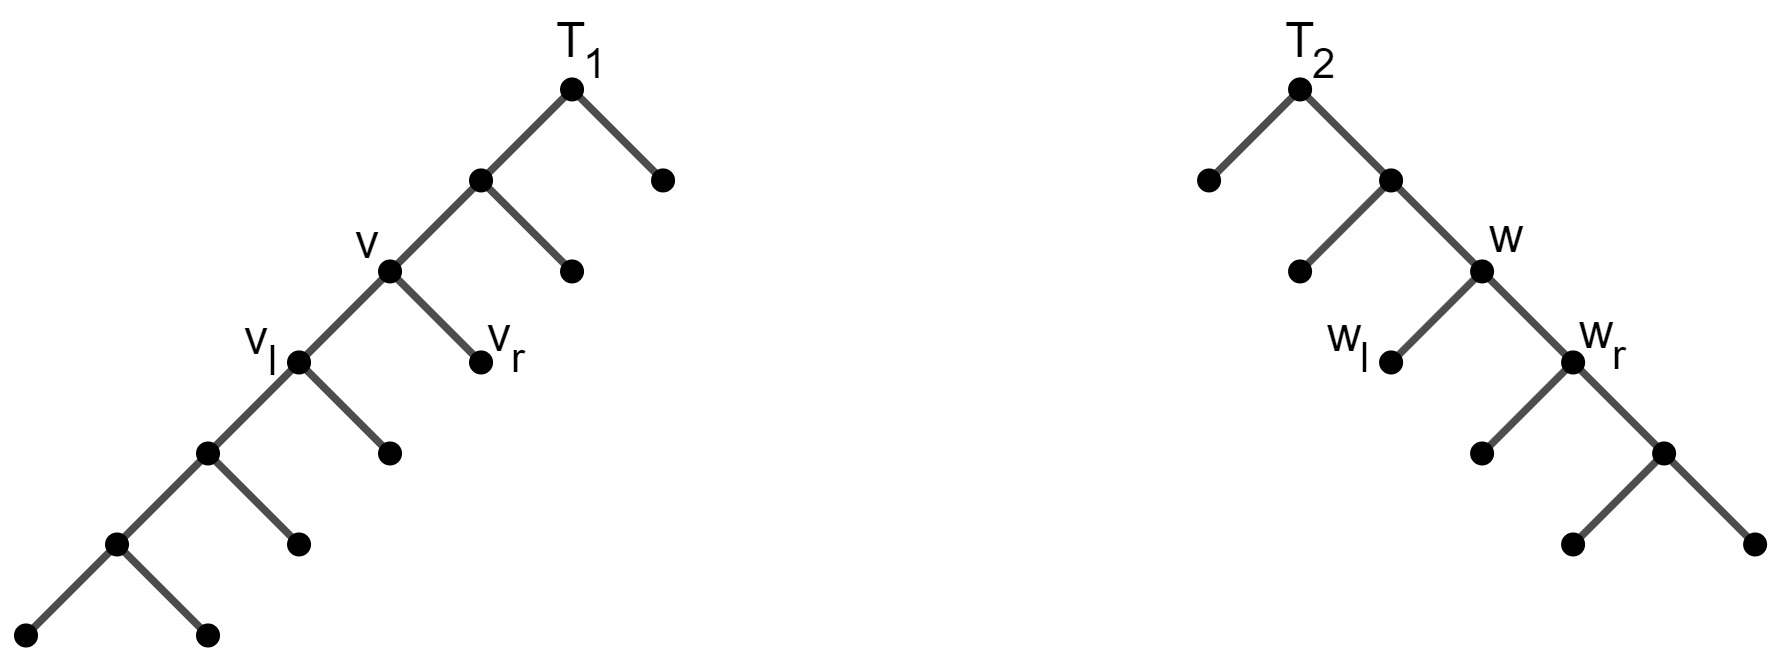
\includegraphics[height=2.5cm]{figures/O(m^2n).JPG}
	\caption{Sketch of $T_1$ and $T_2$ which fulfill a lower bound on the running time for each decomposition algorithm of $\Omega (t_2^2t_1)$}
	\label{fig:m^2n}
\end{figure}
\begin{proof}
Let $S$ be the strategy of decomposition algorithm and assume $T_1$ and $T_2$ to be as in Figure~\ref{fig:m^2n}. As previously stated, every pair $((T_1)_v^{\circ}, (T_2)_w^{\circ})$ for $v \in T_1, w \in T_2$ is a relevant subproblem for $S$. We count the number of such relevant
subproblems, where  $v$ and $w$ are inner nodes of $T_1$ and $T_2$. For an inner node $x$, let us denote the left child of $x$ as $x_l$ and the right child of $x$ as $x_r$. In the forest $(T_1)_v^{\circ}$ the rightmost root is $v_r$ and in $(T_2)_w^{\circ}$ the leftmost root is $w_l$. In each step $S$ decides the direction from which side we should delete. Every
time the strategy chooses left, we delete from $T_1$ and otherwise from $T_2$. This computational approach always keeps $v_r$ as rightmost and $w_l$ as leftmost roots of their respective forests until they are the only nodes left. So it takes at least $\min \{|(T_1)_v^{\circ}|,|(T_2)_w^{\circ}|\}$ steps until every relevant subproblem of $((T_1)_v^{\circ}, (T_2)_w^{\circ})$ is found. Since $v_r$ and $w_l$ are the outermost roots, the computational paths of $((T_1)_v^{\circ}, (T_2)_w^{\circ})$ and $((T_1)_{v'}^{\circ}, (T_2)_{w'}^{\circ})$ are completely disjoint. Because of their structure there are $\frac{t_1}{2}$
and $\frac{t_1}{2}$ internal nodes in $T_1$ and $T_2$ respectively, yielding the following equation:
$$ \sum_{(v,w) \text{internal nodes}}\min \{|(T_1)_v^{\circ}|,|(T_2)_w^{\circ}|\} = \sum_{i=1}^{\frac{t_1}{2}} \sum_{j=1}^{\frac{t_2}{2}} \min \{2i, 2j\} = \Omega(t_2^2 t_1).$$
\end{proof}
In the case of $t_2 \neq \Theta(t_1)$ this bound doesn't match the running time of Demaine et al.'s algorithm. But considering trees structured as the ones in Figure~\ref{fig:m^2nlogm/n}, one can proof the actual lower bound of  $\Omega(t_2^2t_1(1+\log \frac{t_1}{t_2}))$
\begin{figure}[]
	\centering
	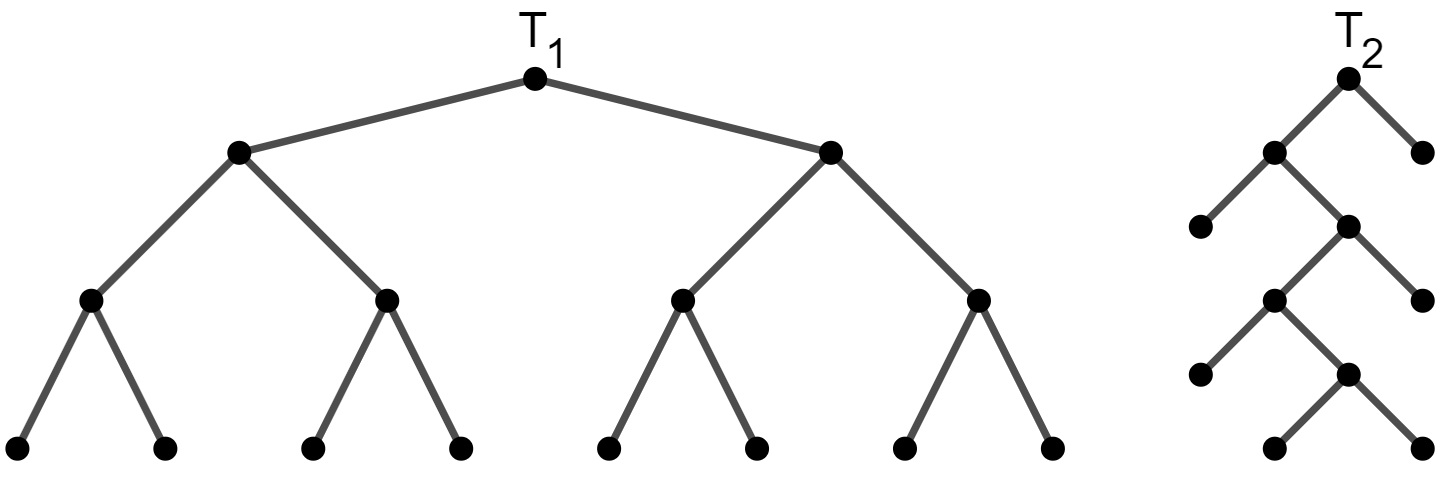
\includegraphics[height=2.5cm]{figures/O(m^2nlogn_m).JPG}
	\caption{$T_1$ and $T_2$ used to prove a lower bound of $\Omega(t_2^2t_1(1+\log \frac{t_1}{t_2}))$}
\label{fig:m^2nlogm/n}
\end{figure}